\documentclass[10pt,a4paper]{article}

% Two-page mini-project report. Compile from this folder: pdflatex report.tex
\usepackage[margin=20mm]{geometry}
\usepackage[T1]{fontenc}
\usepackage{lmodern}
\usepackage{microtype}
\usepackage{graphicx}
\usepackage{booktabs}
\usepackage{amsmath}
\usepackage[colorlinks=true,urlcolor=blue!55!black,linkcolor=blue!55!black,citecolor=blue!55!black]{hyperref}
\usepackage{xcolor}
\setlength{\parindent}{0pt}
\setlength{\parskip}{4pt}
\setlength{\textfloatsep}{9pt}
\setlength{\intextsep}{9pt}
\renewcommand{\refname}{References}

\begin{document}

\begin{center}
{\Large\bfseries Predicting Concrete Compressive Strength from Mix Design\\ with Regularised Polynomial Regression\par}
\vspace{5pt}
{\normalsize Bui Quoc Bao (G2609601D)\par}
\vspace{2pt}
{\small Course: Machine Learning Mini-Project \quad | \quad GitHub: \url{https://github.com/baobqnuce/concrete-strength-ml}\par}
\end{center}
\vspace{-6pt}

\section{Problem and Motivation}
The 28-day compressive strength $f'_c$ is the main acceptance criterion for structural concrete.
To measure it, specimens must be cured and crushed. This takes weeks, and every trial mix
needs a new batch. A model that estimates $f'_c$ from the mix proportions and the age can
screen candidate mixes before laboratory testing and give an early estimate of strength
gain. This matters more for modern mixes with fly ash, slag and superplasticiser,
whose strength development is non-linear and not well described by water--cement-ratio rules.
\textbf{Input:} $\mathbf x\in\mathbb R^8$ (seven constituents in kg/m$^3$ and age in days).
\textbf{Output:} $f'_c$ in MPa.
We study how far the linear-regression methods of the course can go on this task, and
we evaluate them in a way that does not overstate their accuracy.

\section{Dataset and Method}
\textbf{Data.} We use the UCI \emph{Concrete Compressive Strength} dataset~\cite{yeh,uci}:
1030 laboratory tests, $f'_c\in[2.3,\,82.6]$\,MPa, ages 1--365 days. The tests come from only
\textbf{427 distinct mix designs}, because each mix is tested at several ages. Rows from the same
mix are strongly correlated. A random split would therefore place the same mix in both the
training and the test data (data leakage). We assign each mix design to a group and use
\emph{grouped} splitting throughout: 80\% development (815 rows, 341 mixes) and 20\% test
(215 rows, 86 mixes), with seed 42. The test set is used only once.

\textbf{Models.} All models are linear in the parameters:
$\hat y = \mathbf w^\top\boldsymbol\phi(\mathbf x)$.
(i) Ordinary least squares (OLS) on the raw features.
(ii) OLS with age replaced by $\log(\text{age})$, because strength gain is roughly logarithmic in time.
(iii) Polynomial feature expansion $\boldsymbol\phi$ of degree $M$ (44 terms for $M=2$), fitted with
ridge regression, $\min_{\mathbf w}\lVert\mathbf y-\Phi\mathbf w\rVert_2^2+\alpha\lVert\mathbf w\rVert_2^2$,
whose solution $\mathbf w^\star=(\Phi^\top\Phi+\alpha I)^{-1}\Phi^\top\mathbf y$ is unique for every $\alpha>0$.
(iv) Lasso with the $\ell_1$ penalty.
The features are standardised before and after the expansion to keep $\Phi^\top\Phi$ well conditioned.
A gradient-boosting regressor~\cite{sklearn} with default settings serves as a non-linear reference.
The hyper-parameters $(M,\alpha)$, with $M\in\{1,\dots,5\}$ and 15 values $\alpha\in[10^{-4},10^{3}]$,
are selected by \emph{grouped} 5-fold cross-validation on the development set using validation RMSE.
The chosen model is then refit on the full development set and evaluated on the test set (RMSE, MAE, $R^2$).
To check how much the result depends on a single split, the whole procedure (split, selection, test)
is repeated for 10 random seeds.

\section{Results and Discussion}
Grouped CV selects $M=2$ with $\alpha\approx0.3$, i.e.\ almost no shrinkage is needed at this degree.
Fig.~\ref{fig:res}a shows the bias--variance trade-off. Without regularisation, the training error keeps
falling as $M$ grows, while the validation RMSE rises from 6.5 MPa ($M=2$) to above $10^2$\,MPa for $M\ge4$.
This is over-fitting, made worse by extrapolation in the 8-dimensional input space. Ridge keeps the
validation error at 7--9\,MPa for the same degrees, but no degree above 2 beats $M=2$.
Lasso chose the smallest penalty in its grid and kept all 44 terms, so the $\ell_1$ penalty gives no sparsity here.

\begin{table}[h]
\centering
\caption{Validation (grouped 5-fold CV, development set) and test metrics, seed-42 split. Right: test metrics as mean $\pm$ std over 10 grouped splits.}
\label{tab:res}
\small
\begin{tabular}{lcccc|cc}
\toprule
 & Val.\ RMSE & \multicolumn{3}{c|}{Test (seed 42)} & \multicolumn{2}{c}{Test, 10 splits} \\
Model & (MPa) & RMSE & MAE & $R^2$ & RMSE & MAE \\
\midrule
Mean predictor          & 16.30 & 18.04 & 14.67 & 0.00  & -- & -- \\
OLS, raw age            & 10.47 & 10.74 & 8.38  & 0.645 & -- & -- \\
OLS, $\log(\text{age})$ & 7.30  & 7.36  & 5.42  & 0.833 & $7.34\pm0.43$ & $5.69\pm0.39$ \\
Ridge, $M=2$ (selected) & 6.45  & 7.44  & 5.24  & 0.830 & $7.19\pm0.91$ & $5.19\pm0.43$ \\
Gradient boosting (ref.)& 6.23  & 6.34  & 4.31  & 0.876 & $5.93\pm0.52$ & $4.23\pm0.51$ \\
\bottomrule
\end{tabular}
\end{table}

\begin{figure}[h]
\centering
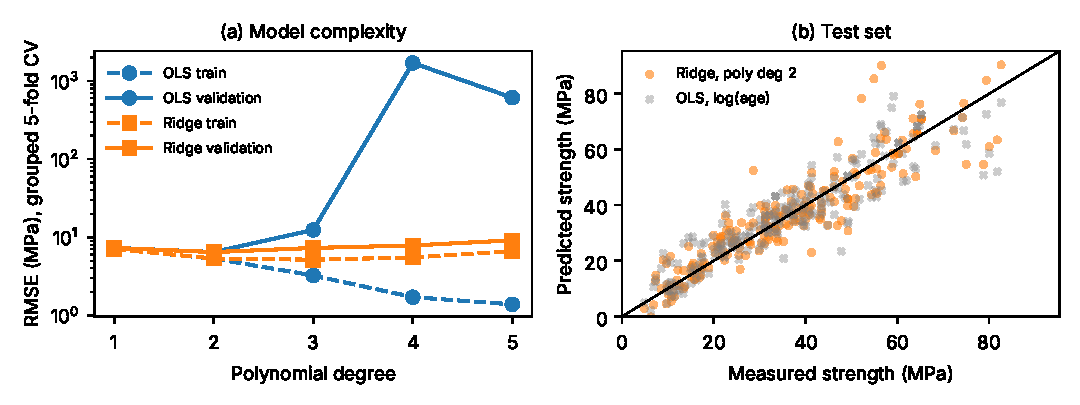
\includegraphics[width=0.9\linewidth]{../results/figures/results.pdf}
\vspace{-4pt}
\caption{(a) Train/validation RMSE (grouped 5-fold CV, log scale) versus polynomial degree, for OLS and for ridge with the best $\alpha$ at each degree. (b) Predicted versus measured strength on the test set.}
\label{fig:res}
\end{figure}

Table~\ref{tab:res} shows that the biggest gain comes from \textbf{domain knowledge}. Replacing age by
$\log(\text{age})$ reduces the test RMSE from 10.7 to 7.4\,MPa and raises $R^2$ from 0.65 to 0.83.
The quadratic ridge model lowers the validation RMSE further (6.45 vs.\ 7.30\,MPa) and the MAE
(5.2 vs.\ 5.7\,MPa over 10 splits). Its test RMSE, however, is not consistently better and varies more
($\pm0.91$ vs.\ $\pm0.43$). Fig.~\ref{fig:res}b explains why: the model is accurate for typical mixes,
but a few mixes are missed by 20--34\,MPa (mostly over-predictions of 52--57\,MPa specimens). The quadratic terms extrapolate
poorly at the edge of the data, and RMSE penalises these large errors heavily.
Gradient boosting is best (RMSE $5.9\pm0.5$\,MPa, $R^2\approx0.87$). This shows that the remaining error is
partly model bias (interactions that a degree-2 polynomial cannot express) and not only measurement noise.
\textbf{Leakage check:} on the development set, random 5-fold CV reports 5.76\,MPa (ridge) and
4.23\,MPa (boosting), versus 6.45 and 6.23\,MPa with grouped folds. A random split would therefore make the
error look up to 32\% smaller, and would favour the more flexible model even more.

\section{Conclusions and Reflection}
A linear model on 8 mix-design inputs predicts concrete strength on unseen mixes with an RMSE of about
7\,MPa ($R^2\approx0.80$--$0.83$). Using $\log(\text{age})$ as a feature matters more than adding
polynomial capacity. Polynomial features help typical predictions, but they need regularisation, and they
remain unreliable when extrapolating. The main methodological lesson is that the validation design matters
as much as the model. Because the rows are not independent, only grouped validation gives an honest estimate of the
generalisation error.
\textbf{Limitations:} the data come from one source with laboratory curing. An error of 6--7\,MPa is useful
for screening mixes but not for structural acceptance. The model gives no uncertainty estimate and should not be
used outside the training ranges (the inference script flags such inputs).
\textbf{Relevance and next steps:} the same workflow (physics-informed features, grouped validation by
specimen or batch) carries over directly to non-destructive testing. For example, in-situ strength could be
estimated by adding ultrasonic pulse velocity or rebound number as inputs. This would turn a mix-design
prior into a monitoring tool for existing structures.

\section*{Reproducibility and Disclosures}
Code, exact commands, the data checksum, the seed and all outputs are provided in the GitHub repository
linked above (\texttt{python -m src.train}; \texttt{python -m src.predict examples/new\_mixes.csv}).
No pretrained models were used. Generative AI (Claude, Anthropic) assisted in writing the code.

\begin{thebibliography}{9}\setlength{\itemsep}{0pt}\small
\bibitem{yeh} I.-C.\ Yeh. Modeling of strength of high-performance concrete using artificial neural networks. \emph{Cement and Concrete Research}, 28(12):1797--1808, 1998.
\bibitem{uci} I.-C.\ Yeh. \emph{Concrete Compressive Strength} [dataset]. UCI Machine Learning Repository, 2007. \url{https://doi.org/10.24432/C5PK67}
\bibitem{sklearn} F.\ Pedregosa et al. Scikit-learn: Machine learning in Python. \emph{JMLR}, 12:2825--2830, 2011.
\end{thebibliography}

\end{document}
